\documentclass[a4paper]{report}
\usepackage[14pt]{extsizes}
\usepackage[utf8]{inputenc}
\usepackage[english,russian]{babel}
\usepackage[OT1]{fontenc}
\usepackage{setspace, amsmath}
\usepackage{amsfonts}
\usepackage{amssymb}
\usepackage[left=20mm, top=10mm, right=15mm, bottom=20mm, nohead, footskip=10mm]{geometry}

\usepackage{graphicx} 
\graphicspath{{images/}}
\DeclareGraphicsExtensions{.pdf,.png,.jpg}

\renewcommand{\theenumi}{\arabic{enumi}}
\renewcommand{\labelenumi}{\arabic{enumi}}
\renewcommand{\theenumii}{.\arabic{enumii}}
\renewcommand{\labelenumii}{\arabic{enumi}.\arabic{enumii}.}
\renewcommand{\theenumiii}{.\arabic{enumiii}}
\renewcommand{\labelenumiii}{\arabic{enumi}.\arabic{enumii}.\arabic{enumiii}.}
\usepackage{indentfirst}
\usepackage{fontspec}
\setmainfont{Times New Roman}

\begin{document}
\begin{titlepage}
\newpage



\begin{center}
\vfill
%\framepage

Федеральное государственное бюджетное образовательное учреждение высшего образования «МИРЭА — Российский технологический университет»\\
\ \\

\hfill\vbox
{
\hbox{Кафедра высшей математики}
}

\vfill

{\large\bf Разработка безопасного аудиокодека с шифрованием трафика\\}
\ \\
Реферат студентов 1 курса института искусственного интеллекта\\
Коровяковского Степана и Урвачева Романа

\vfill

%{
%\hbox{Научный руководитель:}
%\hbox to 16cm {к.т.н, доцент \hrulefill Х.З.~Мамаев}
%\hbox{}
%\hbox{Заведующий кафедрой:}
%\hbox to 16cm {д.ф.-м.н., профессор \hrulefill В.С.~Луговской}
%}

\vfill

Москва 2022
\end{center}

\end{titlepage}
\tableofcontents
\newpage
\chapter*{Введение}
\chapter{Изучение способов передачи аудиоданных в информационно-телекоммуникационных сетях}
\section{Телекоммуникационные технологии}
Каждому поколению свойственно разрабатывать новые технические средства, совершенствовать систему учета, обработки, передачи и хранения данных. Первыми телекоммуникационными средствами признан телеграф, телефон, телетайп, радиоприемник. Середина XIX столетия отмечена массовым использованием спутниковой связи, вычислительной техники, компьютерной сети. В результате это положительно отразилось на развитии новых телекоммуникационных технологий.
\par Современный мир невозможен без телекоммуникационных технологий, которые стирают государственные границы и расстояние между людьми, делают доступной мобильную и видеосвязь и позволяют решать множество задач в сфере управления, образования, коммерции. Каждый человек сталкивается с ними ежедневно, деля телефонные звонки, проверяя почту или покупая товары в интернет-магазинах.

\subsection{Определение и понятие телекоммуникационных \\ технологий}
Общее понятие информационных и коммуникационных технологий включает в себя совокупность методов, процессов и устройств, позволяющих получать, собирать, накапливать, хранить, обрабатывать и передавать информацию, закодированную в цифровом виде или существующую в аналоговом виде.
\par В более узком смысле под телекоммуникационными технологиями понимается совокупность программных и аппаратных средств, позволяющих устанавливать связь без использования проводов и передавать пакеты информации.

\subsection{Виды телекоммуникационных технологий}
Телекоммуникационные технологии могут быть рассмотрены как сервисы, предоставляемые провайдерами различного уровня.
По этому принципу можно выделить следующие виды телекоммуникационных технологий:
\begin{itemize}
\item телефонная связь, современная телефонная связь позволяет легко переключаться с аналогового стандарта на цифровой, подключать к интернет городские телефоны и соединять в одну сеть аналоговые и мобильные устройства;
\item радиосвязь, которая сегодня превратилась в сотовую связь, телефон, перемещаясь в пределах сети, оказывается в зоне действия различных передающих устройств;
\item спутниковая связь, которая используется провайдерами для создания систем мобильной связи и для государственных систем связи;
\item интернет – наиболее распространенный вид телекоммуникационных технологий, при которых подключение к сети может осуществляться как проводным, так и беспроводным способом.
\end{itemize}

\subsection{Основные типы информационно-телекоммуникационных сетей}
Телекоммуникационные технологии, используемые в интернете, сейчас переживают этап бурного развития и роста. С каждым днём создаётся всо больше и больше новых сетей различных типов, среди которых основными являются:
\begin{itemize}
\item локальные сети компаний или учреждений (Local Area Network - LAN), связь между компьютерами в них осуществляется и проводным и беспроводным способом, количество пользователей этих сетей ограничено. Локальные сети могут быть корпоративными, в некоторых странах создаются и городские локальные сети;
\item глобальные сети (Wide Area Network – WAN) представляют совокупность большого количества узлов-компьютеров, расположенных в разных странах мира и связанных между собой каналами оптово-волоконной связи. К этим сетям, представляющим услуги провайдеров, подключаются локальные сети.
\end{itemize}

\subsection{Технические и программные средства \\ телекоммуникационных технологий}
Работоспособность интернета основана на использовании сетевых узлов и каналов связи. К узлам относятся как отдельные компьютеры, так и хостинги, предоставляющие IP-адреса и доменные имена.
Каналы связи делятся на 4 типа:
\begin{itemize}
\item аналоговые телефонные сети;
\item провода, по которым передается электричество;
\item оптоволоконные каналы связи;
\item беспроводные каналы связи, модемные или спутниковые.
\end{itemize}
К телекоммуникационным каналам связи относятся, в основном, третий и четвертый типы.

Среди коммуникаций, используемых для организации связи, можно отдельно отметить программы, обеспечивающие работу телекоммуникационного оборудования такого, как:
\begin{itemize}
\item IP-АТС;
\item маршрутизаторы;
\item компьютеры.
\end{itemize}

\subsection{Программное обеспечение телекоммуникационных \\ технологий}
Для передачи данных с использованием возможностей телекоммуникационных технологий применяется специальное программное обеспечение. Это обеспечение функционирует по определенным протоколам или по механизмам, разработанным с целью упростить и стандартизировать работу всех узлов сети, выстроив ее по единому алгоритму.

Так, для передачи по компьютерным сетям разработан стандарт MIME (ssr-Multipurpose Internet Mail Extensions), переводящий данные в формат понятный почтовому серверу. Общение компьютера пользователя и сервера происходит в виде диалога в режиме Клиент-Сервер, где с каждой стороны его участником является определенная программа.

Отдельные программы используются для работы мессенджеров, которые позволяют обмениваться сообщениями, совершать телефонные звонки с передачей голосовой и видеоинформации. Здесь происходит коммуникация не только компьютер - почтовый сервер, к диалогу подключаются и телефонные станции.

\subsection{Основные задачи сетевых телекоммуникационных технологий}
Различные сетевые телекоммуникационные технологии позволяют решать такие задачи, как:
\begin{itemize}
\item передачу информации в необходимых форматах;
\item выстраивание коммуникаций;
\item обеспечение взаимодействия различных участников сети.
\end{itemize}

Среди новых технологий особое место занимают программы, позволяющие работать в режиме нетворкинга, объединение CRM-систем с возможностями социальных сетей и многое другое.

Создание корпоративных сетей как офисных, компьютерных, так и телефонных, также попадает в область сетевых технологий, призванных обеспечить синергию за счет эффективной коммуникации пользователей.

\subsection{Технологии защиты информации в телекоммуникационных сетях}
Большая часть информационных массивов, принадлежащих государственным учреждениям и коммерческим предприятиям, имеет самостоятельную ценность и является добычей для потенциальных похитителей, которыми могут быть и хакеры, и внутренние пользователи.

Для защиты информации от утечек разработаны сложные программные продукты, позволяющие определить проникновение неавторизованного пользователя или вируса-похитителя информации в сеть и блокировать его.

Существуют специальные стандарты защиты информации, но даже они не всегда могут уберечь сети от взлома и хищения данных. Особенно уязвимы компьютеры и мобильные устройства частных пользователей, использующих только антивирусы.

От хищения информации с помощью закладных устройств, перехватывающих электромагнитные излучения, необходимо бороться при помощи технических средств.

\subsection{Использование телекоммуникационных технологий}
Телекоммуникационные технологии сегодня в основном применяются для организации систем связи.

Но сами системы связи имеют прикладное значение, при помощи этих технологий можно достичь существенно более важных целей, среди которых:
\begin{itemize}
\item создание систем дистанционного обучения;
\item обеспечение недорогой голосовой телефонной связи;
\item создание информационных систем предприятий и объединение их в комплекс, позволяющий оптимизировать управление;
\item построение банковских сетей;
\item проведение электронных аукционов и тендеров для обеспечения государственных закупок;
\item осуществление коммуникации удаленных субъектов;
\item для интернет-торговли;
\item осуществление дистанционного управления в государственной и в частной сфере.
\end{itemize}

Спектр возможностей использования телекоммуникационных технологий расширяется с каждым днем. Сложно сказать, что именно будет предложено завтра в этой области, чтобы сделать связь доступнее, а производственные процессы – проще.

\section{Описание способов передачи аудиоданных}
\subsection{Телефонные каналы связи}

Взаимное проникновение вычислительной техники и технических средств связи оказало серьезное влияние как на структуру компьютеров, так и на структуру каналов связи.

Средства связи, предназначенные для передачи информации между людьми, имеют длительную историю, развитую структуру (в мировом масштабе), мощную научную и технологическую базу и, начиная с 60-х годов, стали использоваться для передачи данных, т.е. для передачи информации между техническими средствами вычислительной техники, что потребовало включения в каналы связи дополнительных технических ус тройс тв.

В настоящее время для распределенных вычислительных систем наиболее широко используются телефонные каналы.

На рис. 1.1 представлена упрощенная схема линии аналоговой междугородней телефонной связи.

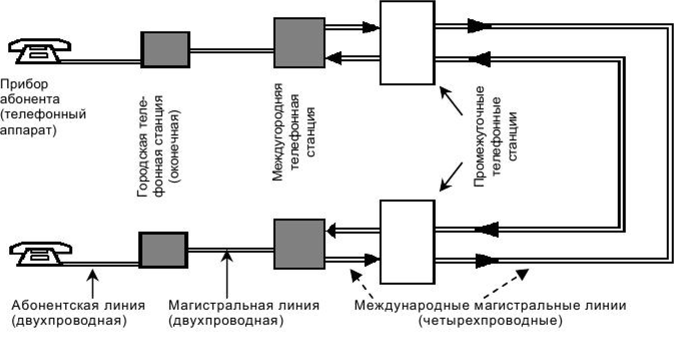
\includegraphics[scale=1.4]{66}
{\centering\caption{Рис. 1.1 Схема междугородней телефонной связи}\\}
~

На участке от телефонного аппарата до местной АТС происходит передача в первичной полосе частот « 200 - 3100 Гц (полоса частот человеческого голоса). При этом от каждого аппарата до АТС проводится двухпроводная электрическая линия для передачи этого сигнала, в дальнейшем происходит преобразование его в иную форму с целью уплотнения передачи. В каждом из последующих каналов идет очень большое количество передач. Существует два типа уплотнения: частотное и временное. В традиционных линиях связи, как правило, используется частотное уплотнение.

Сущность частотного уплотнения для грех абонентов представлена на рис. 4.2.

\bigskip
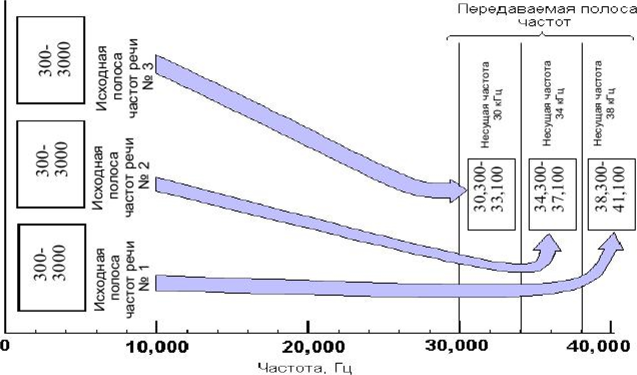
\includegraphics[scale=1.4]{67}
{\centering\caption{\newline Рис. 1.2 Частотное уплотнение телефонных каналов}\\}
~

Передаваемый сигнал на входе в магистральную линию «смешивается» с так называемой несущей (более высокой) частотой и одновременно с другими сигналами (которые передаются на других несущих частотах) распространяется по магистралям. На выходе передаваемые сигналы выделяются из несущих частот и по индивидуальным линиям доставляются абоненту.

Процедура на входе в магистральные линии связана с различного вида модуляцией несущих частот, а обратное преобразование на выходе из магистральных линий, соответственно, с демодуляцией.

Модуляция несущей - изменение ее амплитуды, частоты, фазы или комбинации этих характеристик в соответствии с передаваемым сигналом.

Использование описанных средств связи для передачи данных, т.е. замена абонента-человека на техническое устройство (ЭВМ), требует включения в эту систему дополнительных устройств, адаптирующих информационные СОД к передаче по каналу связи.






\end{document}





